\section{Digital Teori}
\textit{Noget om denne section?}

\subsection{CY8CKIT-043 PSoC 4-M og PSOC Creater}
Til dette projekt anvendes CY8CKIT-043 Programmable System on Chip (PSoC) 4 M-Series Prototyping Kit og programmet PSoC Creater i den digitale del til at opsamle det biologiske signal.\\
CY8CKIT-043 PSoC 4 M-Series Prototyping Kit er en prototyping platform, der indeholder tre mikroprocessorer: to Programmable System-on-Chips (PSoC) og en Programmable Radio on Chip (PRoC), hvilket ses på \figref{fig:PSoC}. Den første PSoC LP5 på mikrokontrolleren sidder på KitProg boardet og kan indeholde programmer, der kan indlæses på en computer ved hjælp af USB stikket. Den bruges til at programmere og debug softwaren på target boardet af mikrokontrolleren, hvorfor denne del kan knækkes af resten af stikket og fungere selvstændigt. Dette kræver dog, at softwaren først er programmeret på den anden mikroprocessorer, som er PSoC 4200M. Denne fungerer som hovedcomputeren, der programmeres på igennem c koden, og muliggøre eksempelvis høj-performans analog til digital konvertering igennem sin 12-bits SAR ADC. På bagsiden af mikrokontrolleren sidder en PRoC med Bluetooth Low Energy(BLE). Denne PRoC har ikke lige så mange muligheder for afbenyttelse i forhold til PRoC 4200M, da BLE optager meget plads, hvorfor der ikke er plads til meget andet. \citep{CYPRESS2016PSoC,Semiconductor2016,CYPRESS2016Cortexm0}
\begin{figure}[H]
	\centering
	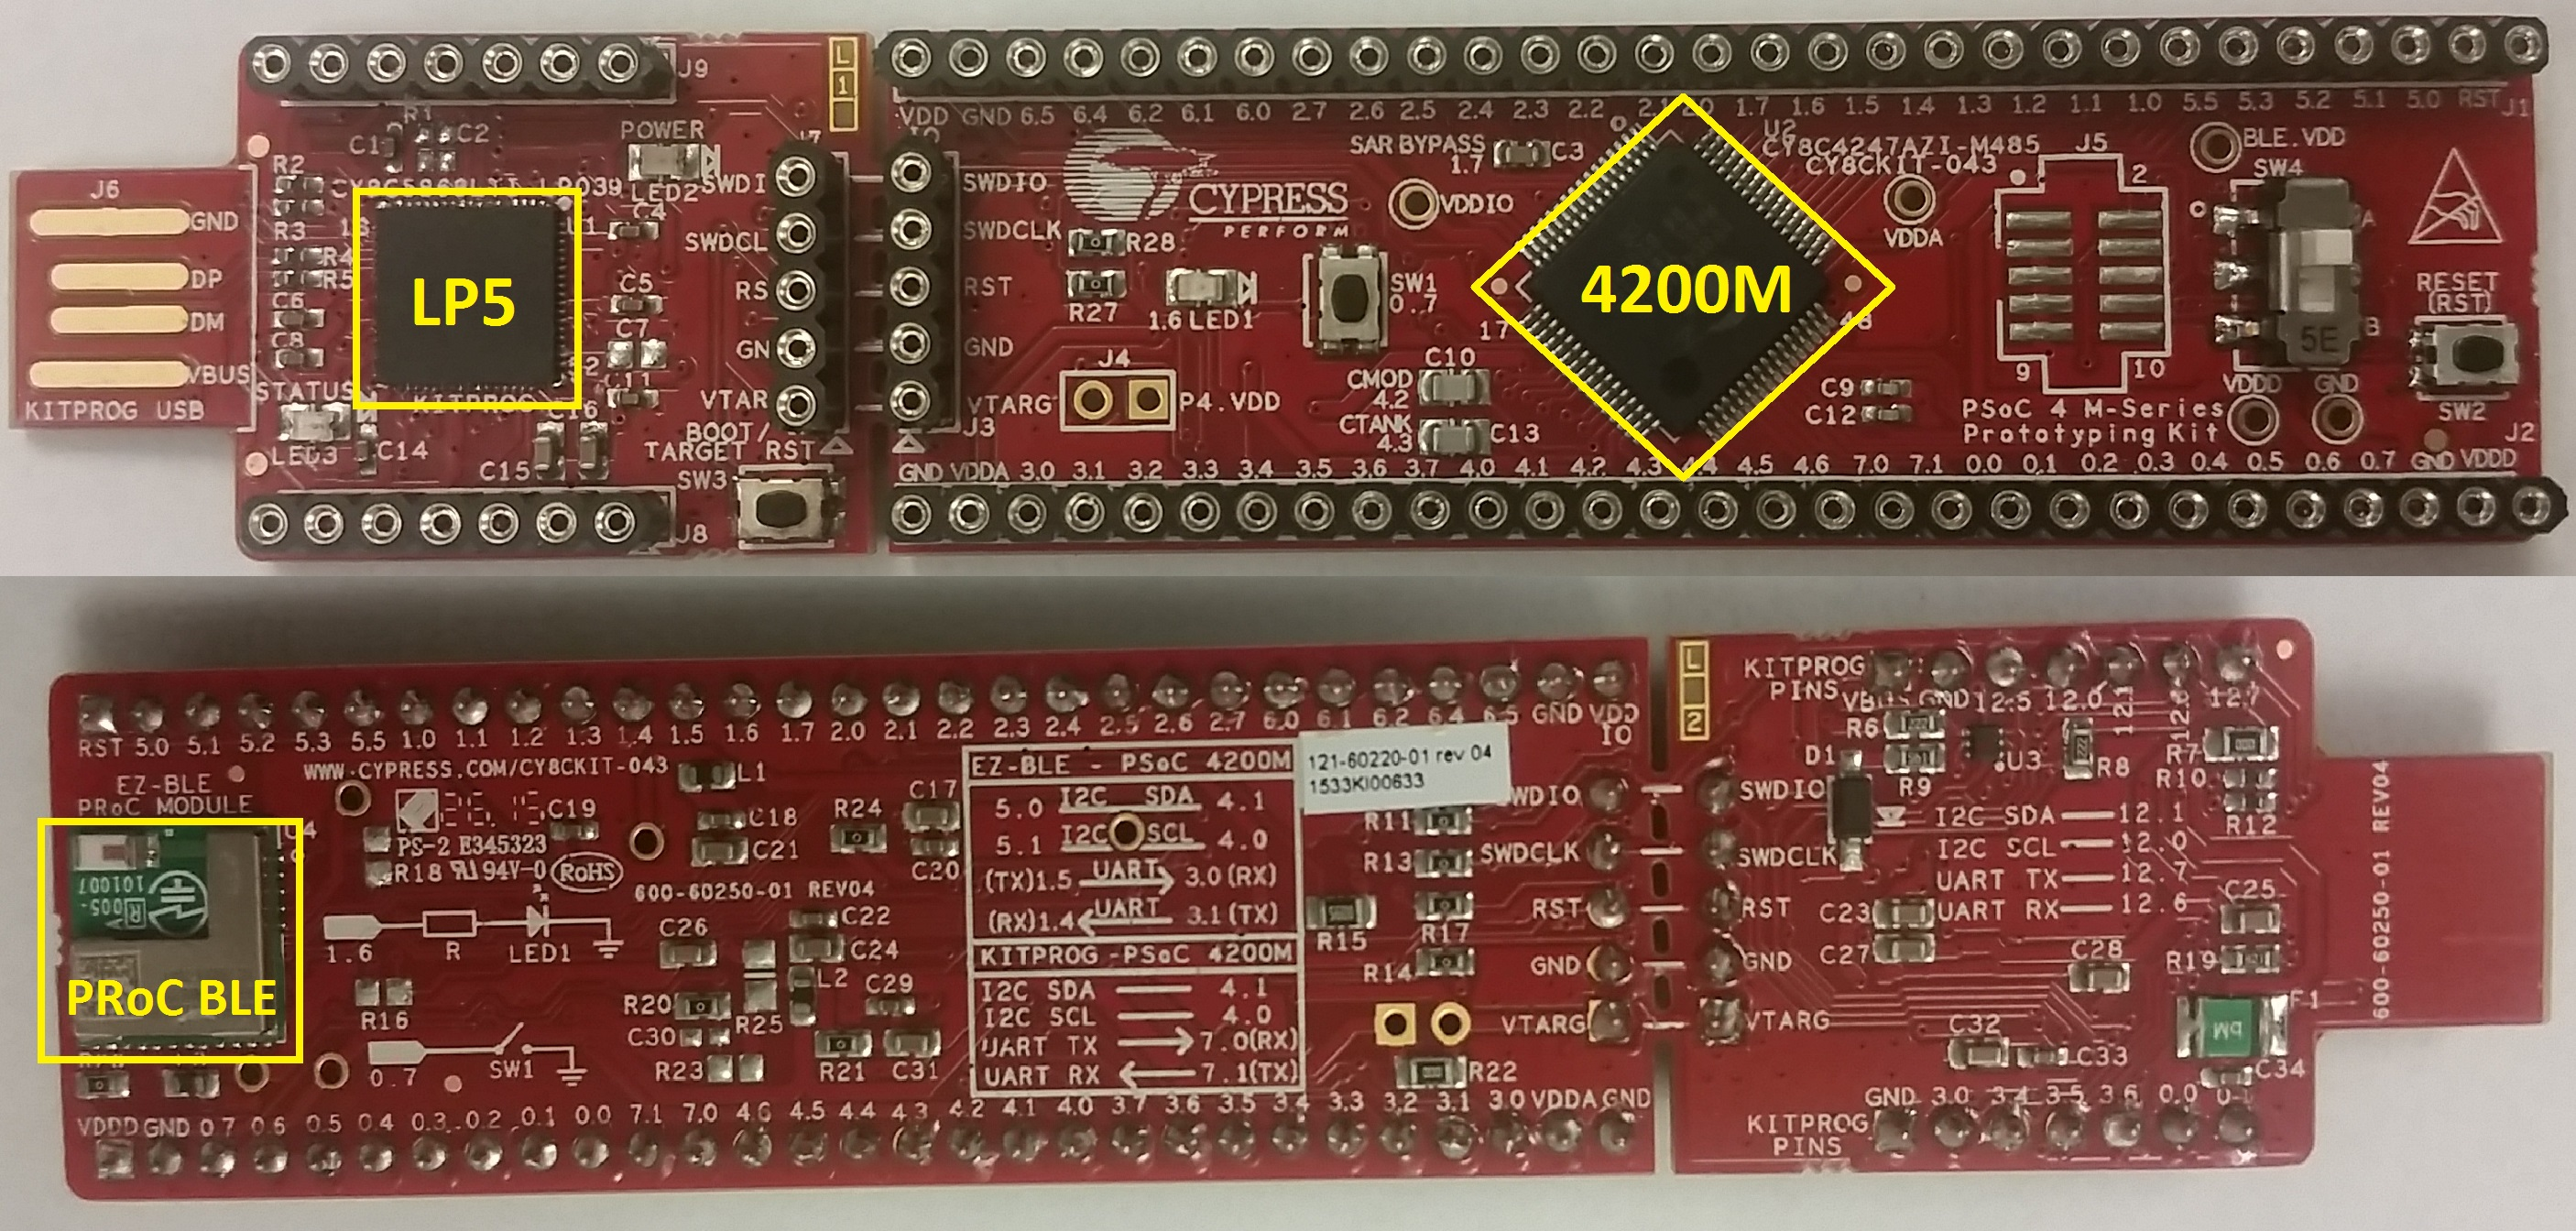
\includegraphics[scale=0.15]{figures/bProblemloesning/PSoC3.jpg}
	\caption{På figuren ses mikrokontrolleren CY8CKIT-043 PSoC 4 M-Series Prototyping Kit foran og bagpå. På forsiden findes to PSoC og på bagsiden findes PRoC, som alle er tydeliggjort med gul markering og navngivning. Mikrokontrolleren kan knækkes over i to: KipProg board med USB stik og target board med hovedchippen PSoC 4200M\fxnote{Navnene er fundet nederst på side 26 i manualen}. PRoC'en er ikke påmonteret som standart fra Cypress, hvorfor denne er blevet loddet manuelt på efterfølgende. Kontakten helt til højre på forsiden af target boardet, som også er loddet manuelt på efterfølgende, skal trykkes ned for, at PRoC programmeres på istedet for PSoC 4200M. \citep{CYPRESS2016PSoC,Semiconductor2016}}
	\label{fig:PSoC}
\end{figure}
Når data skal opsamles, skal to CY8CKIT-043 PSoC 4 M-Series Prototyping Kit benyttes. Én skal placeres på personen og opsamle data, som skal sendes til en anden mikrokontroller, der er koblet til en computer via USB. Dette kan lade sig gøre, da mikrokontrolleren har Inter-Integrated Circuit (I$^{2}$C) interface. I$^{2}$C er en computerbus dataprotokol, hvilket gør det muligt for de to mikrokontrollere at opføre sig som master eller slave. Rollen i kredsen bestemmes igennem softwaren. Masteren kontrollerer I$^{2}$C bussen og sender kommandoer til slaven. Både master og slave kan sende og modtage data, men masteren kontrollerer, hvornår dette kan finde sted. Det er muligt med I$^{2}$C interface at lave flere slaver eller flere masters til slaverne. I dette tilfælde vil der være én slave og én master. Disse kan kommunikere ved hjælp af et virtuelt kabel, som skabes af BLE. \citep{Semiconductor2016,Sparkfun2016}\\
Mellem PSoC LP5 og PSoC 4200M samt mellem PSoC 4200M og PRoC findes blandt andet nogle serielle porte med to ledninger til at modtage data (RX) og sende data (TX). Disse tre mikroprocessorer kommunikerer altså ikke på samme måde, som to mikrokontrollere kommunikerer med hinanden. \citep{Semiconductor2016} \\
Mikrokontrolleren kræver en ekstern strømkilde for at kunne fungere. Igennem USB porten adapteres tilslutningen til 5V, men det er muligt at tilkoble en strømkilde til boardets lav-volt applikation, hvilket gør den trådløs. 3,3V til 5,5V tilsluttes VDD fra en reguleret forsyning, hvilket er yderst essentielt, da boardet ikke besidder en elektrostatisk afladnings beskyttelse (ESD). Hvis en ekstern strømforsyning til VDD er for ustabil eller af dårlig kvalitet, kan mikrokontrollerens kredsløb blive forstyrret og vil derved ikke fungere optimalt. \citep{Semiconductor2016}

Programmet PSoC Creater kan designe hardware og software til mikrokontrolleren. Herigennem bliver rekonfigurerbare analoge blokke og digital programmerbar logik kombineret\fxnote{kan den fysiske hardware opbygges digitalt}, hvorved softwaren kan tilpasses de fysiske komponenter direkte igennem kodedesign. Programmet indeholder forskellige komponenter og kodeeksempler, hvilket kan blive behjælpeligt under algoritmedesignet. \citep{Semiconductor2016} \\
Når mikrokontrolleren er tilsluttet computeren og debugger igennem PSoC Creater, kan matlab fungere som et grafisk bruger interface (GUI). Dette muliggør live visualisering af den data, som eksempelvis en master mikrokontroller modtager fra en slave mikrokontroller.

\subsection{Mikrokontrollerens target CPU}
Target CPU'en på CY8CKIT-043 PSoC 4 M-Series Prototyping Kit er 4200M, som besidder en ARM cortex-M0 processer og har produktnavnet CY8C4247AZI-M485. Denne er basseret på Instruction set architecture (ISA) kategorien Reduced Instruction Set Computer (RISC). ISA beskriver\fxnote{processor design teknikken}, hvordan processoren vil bearbejde dens instruktioner. ISA's kategorier kan blandt andet være complex instrucion set computer (CISC) eller RISC. En CISC baseret computer vil udføre opgaver med så få linjer som muligt. Processorens hardware opbygget til at forstå og udføre komplekse instruktioner, hvilket kræver flere transistorer end RISC metoden. RISC processorer benytter simple instruktioner, som kan forløbe inden for en clock cycle\fxnote{dansk? I så fald klok omgang?}. Derimod kræver dette mere RAM, fordi hver opgave hentes ned og gemmes indtil færdiggjort. Denne metode tillader dog pipelinning, hvilket gør at flere instruktioner kan køre samtidig.\fxnote{fetch - decode - exicute. Mere laves samtidig} Sammenlignet er RISC processen hurtigere end CISC, men CISC computere kan udføre flere komplekse instruktioner på færre linjer end RISC. \citep{CYPRESS2016Cortexm0,Semiconductor20164200M,Yadav2016}\\
CPU'en i Cortex-M0 er en del af det 32-bit microcontroller unit (MCU) delsystem, som optimerer energibesparende drift ved hjælp af clock gating\fxnote{Clock gating saves power by adding more logic to a circuit to prune the clock tree. Pruning the clock disables portions of the circuitry so that the flip-flops in them do not have to switch states. Switching states consumes power. When not being switched, the switching power consumption goes to zero, and only leakage currents are incurred}. %% Noget om deep sleep / low power mode (Hvis den har det), hvor mange registre den har og hvis nogen af dem har dedikerede funktioner
CPU'en har en flash hukommelse på 128 kB og en 16 kB RAM. Algoritmen og dermed programmet for mikrokontrolleren gemmes i flash, da RAM hukommelsen kræver konstant strøm og slettes dermed, hvis strømtilførslen til mikrokontrolleren slukkes. \citep{Semiconductor20164200M}

tilgængelige pins - tilkobling af perifære moduler, som f.eks. en sensor
Mere om ADC'en 12-bits SAR ADC med 1 mega sample pr sekund (Msps) konverterings rate. (se end tial forcing - biofeedback til apopleksi). men ADC virker ikke under deep sleet mode, fordi den kræver høj hastighed clock
oscillatorer - styrer hastigheden på clocks, afhænger af spændingsfrosyning, men der er en 32 kHz (ILO Clock) low power mode (forklar om dette, meget relevant)
output - (se end tial forcing)

\subsection{Interrupts}
Interrupt er en funktion, som kan afbryde main filen for CPU'en, hvis en bestemt hændelse sker eller  - Detektion af diafragma \citep{Badiger2016}

%%%%%%%%%% Clocks
- detektion af diafragma, spilbaseret

%%%%%%%%%% Trådløs kommunikation - Bluetooth
radiomoduler - (Aktivitetsmåler til monitorering)

UART (Aktivitetsmåler til monitorering)



%
%
% I pdf'en for mikrokontrolleren - se side 23
% Skrive om I2C
%
%Denne prototyping Kit platform er ved hjælp af en computer med aktiv bluetooth i stand til at sende og modtage trådløs data fra Y8CKIT-042-BLE Bluetooth® Low Energy (BLE) Pioneer Kit platformen, som indeholder en PRoC.
%CYPRESS2016BLE
%CYPRESS2016PSoC
%Semiconductor2016
%Semiconductor2016BLE